\documentclass[../main.tex]{subfiles}

%\graphicspath{{\subfix{../images/}}}

\begin{document}

\section{{\sc Grau} - Elektrodynamik Aufgabensammlung}
\subsection{Exercise 8.1 - Hertzscher Dipol - NOT DONE YET}
With $\vec{p}_0=q\vec{d}$ and $d\ll r$
\begin{align}
\rho(\vec{r},t)
&=
q\delta(\vec{r}-\frac{\vec{d}}{2} \cos(\omega t))+
(-q)\delta(\vec{r}+\frac{\vec{d}}{2} \cos(\omega t))\\
\rho(\vec{r},t_\text{ret})
&=
q\delta(\vec{r}-\frac{\vec{d}}{2} \cos(\omega (t-\frac{|\vec{r}-\vec{r}'|}{c})))+
(-q)\delta(\vec{r}+\frac{\vec{d}}{2} \cos(\omega (t-\frac{|\vec{r}-\vec{r}'|}{c})))\\
&\simeq
q\delta(\vec{r}-\frac{\vec{d}}{2} \cos(\omega (t-\frac{r}{c})))+
(-q)\delta(\vec{r}+\frac{\vec{d}}{2} \cos(\omega (t-\frac{r}{c})))\\
\end{align}

\begin{align}
\phi(\vec{r},t)
&=\frac{1}{4\pi\varepsilon_0}\int\frac{\rho(\vec{r}',t_\text{ret})}{|\vec{r}-\vec{r}'|}d^3\vec{r}'\\
&=\frac{q}{4\pi\varepsilon_0}\int\frac{\delta(\vec{r}'-\frac{\vec{d}}{2}\cos(\omega [t-\frac{r}{c}]))-\delta(\vec{r}'+\frac{\vec{d}}{2}\cos(\omega [t-\frac{r}{c}]))}{\sqrt{r^2+r'^2-2\vec{r}\cdot\vec{r}'}}d^3\vec{r}'\\
&=\frac{q}{4\pi\varepsilon_0}\int\frac{\delta(\vec{r}'-\frac{\vec{d}}{2}\cos(\omega [t-\frac{r}{c}]))-\delta(\vec{r}'+\frac{\vec{d}}{2}\cos(\omega [t-\frac{r}{c}]))}{r\sqrt{1+\frac{r'^2}{r^2}-2\frac{\vec{r}\cdot\vec{r}'}{r^2}}}d^3\vec{r}'\\
&\simeq\frac{q}{4\pi\varepsilon_0}\int\frac{\delta(\vec{r}'-\frac{\vec{d}}{2}\cos(\omega [t-\frac{r}{c}]))-\delta(\vec{r}'+\frac{\vec{d}}{2}\cos(\omega [t-\frac{r}{c}]))}{r}\left(1+\frac{\vec{r}\cdot\vec{r}'}{r^2}+\frac{r'^2}{r^2}\right)d^3\vec{r}'\\
&=\frac{q}{4\pi\varepsilon_0}\frac{1}{r}\left[\left(1+\frac{\vec{r}\cdot\left[\frac{\vec{d}}{2}\cos(\omega [t-\frac{r}{c}]))\right]}{r^2}\right)-\left(1-\frac{\vec{r}\cdot\left[\frac{\vec{d}}{2}\cos(\omega [t-\frac{r}{c}]))\right]}{r^2}\right)\right]\\
&=\frac{q}{4\pi\varepsilon_0}\frac{1}{r} \frac{\vec{r}\cdot\vec{d}\cos(\omega [t-\frac{r}{c}]))}{r^2}\\
\end{align}

\section{{\sc Zangwill} - Classical Electrodynamics}
\subsection{Exercise 10.1 In-Plane Field of a Current Strip}
We start with the Biot-Savart law (10.15)
\begin{align}
\mathbf{B}(\mathbf{x})=\frac{\mu_0}{4\pi}\int d^3x'\frac{\mathbf{j}(\mathbf{x}')\times(\mathbf{x}-\mathbf{x}')}{|\mathbf{x}-\mathbf{x}'|^3}
\end{align}
with
\begin{align}
\mathbf{j}&=(0,0,K)\delta(x')\Theta(y')\Theta(y'-b)\\
\mathbf{x}-\mathbf{x}'&=(0,a+y',z')^T\\
\mathbf{j}(\mathbf{x}')\times(\mathbf{x}-\mathbf{x}')&=(a+y')K\delta(x')\Theta(y')\Theta(y'-b)
\end{align}
then
\begin{align}
\mathbf{B}(\mathbf{x})
&=\frac{\mu_0K}{4\pi}\int_{-\infty}^\infty dx'\int_0^b dy'\int_{-\infty}^\infty dz'\frac{(a+y')}{\sqrt{(a+y)^2+z'^2}^3}\delta(x')\\
&=\frac{\mu_0K}{4\pi}\int_0^b dy'\int_{-\infty}^\infty dz'\frac{(a+y')}{\sqrt{(a+y')^2+z'^2}^3}\\
&=\frac{\mu_0K}{4\pi}\int_0^b dy'\frac{2}{a+y}\\
&=\frac{\mu_0K}{2\pi}\log\frac{a+b}{a}\\
&=\frac{\mu_0I}{2\pi b}\log\frac{a+b}{a}\\
\end{align}


\section{{\sc Stratton} - Electrodynamgnetic Theory}
\subsection{Problem III.1 Coodinate transform}

\begin{enumerate}[a.]
\item Starting
\begin{align}
\xi+i\eta&=f(x+iy)=f(\alpha(x,y))\\
\rightarrow d\xi+id\eta
&=\frac{\partial f(\alpha)}{\partial\alpha}d\alpha\\
&=\frac{\partial f(\alpha)}{\partial\alpha}\left(\frac{\partial\alpha}{\partial x}dx+\frac{\partial\alpha}{\partial y}dy\right)\\
&=\frac{\partial f(\alpha)}{\partial\alpha}\left(dx+idy\right)\\
&=f'\cdot\left(dx+idy\right)
\end{align}
then calculating the absolute square
\begin{align}
|f'|^2(dx^2+dy^2)&=\frac{1}{h^2}(dx^2+dy^2)\\
&=|d\xi+id\eta|^2\\
&=(d\xi+id\eta)(d\xi-id\eta)\\
&=d\xi^2+d\eta^2
\end{align}
then with $dz=d\zeta$
\begin{align}
ds^2&=dx^2+dy^2+dz^2\\
&=h^2(d\xi^2+d\eta^2)+d\zeta^2
\end{align}

\item The metric is diagonal $g_{ij}=\text{diag}(h^2,h^2,1)$ then
\begin{align}
\mathbf{d\eta}\cdot\mathbf{d\xi}
=(0\,d\eta\,0)\left(\begin{array}{ccc}
h^2 & 0   & 0\\
0   & h^2 & 0\\
0   & 0   & 1
\end{array}\right)
\left(\begin{array}{c}
d\xi\\
0  \\
0  
\end{array}\right)=0
\end{align}

\item 
\begin{enumerate}
\item Let's look at the inverse transformation
\begin{align}
dx&=\frac{1}{2}(\frac{-id\eta+d\xi}{f'^*}+\frac{id\eta+d\xi}{f'})\\
dy&=\frac{1}{2}(\frac{id\eta+d\xi}{f'^*}+\frac{id\eta-d\xi}{f'})
\end{align} 
With the two vectors in cartesian coords
\begin{align}
\mathbf{v}_1=\alpha_1\mathbf{dx}+\beta_1\mathbf{dy}\qquad 
\mathbf{v}_2=\alpha_2\mathbf{dx}+\beta_2\mathbf{dy}
\end{align}
and in the $\xi,\eta$ coords
\begin{align}
\mathbf{v}_1&=\frac{1}{2}\left(\frac{\alpha_1+i\beta_1}{f'^*}+\frac{a_1-i\beta_1}{f'}\right)\mathbf{d\xi}+\frac{1}{2}\left(\frac{-i\alpha_1+\beta_1}{f'^*}+\frac{ia_1+\beta_1}{f'}\right)\mathbf{d\eta}\\
\mathbf{v}_2&=\frac{1}{2}\left(\frac{\alpha_2+i\beta_2}{f'^*}+\frac{a_2-i\beta_2}{f'}\right)\mathbf{d\xi}+\frac{1}{2}\left(\frac{-i\alpha_2+\beta_2}{f'^*}+\frac{ia_2+\beta_2}{f'}\right)\mathbf{d\eta}\end{align}
The angle between to vectors is in both cases given by
\begin{align}
\frac{\langle \mathbf{v}_1,\mathbf{v}_2\rangle}{|\mathbf{v}_1||\mathbf{v}_2|}
=\frac{g_{ij}v_1^iv_2^j}{\sqrt{g_{ij}v_1^iv_1^j}\sqrt{g_{ij}v_2^iv_2^j}}
=\frac{\alpha_1\alpha_2+\beta_1\beta_2}{\sqrt{\alpha_1^2+\beta_1^2}\sqrt{\alpha_2^2+\beta_2^2}}
\end{align}
So the transform conserves angles and therefore does NOT change shapes.


\item Let's calculate the Laplace-Beltrami operator with $|g|=h^2$ and $g^{-1}=\text{diag}(h^{-2},h^{-2},1)$
\begin{align}
\Delta&=\frac{1}{\sqrt{|g|}}\partial_i\left(\sqrt{|g|}g^{ij}\partial_j\right)\\
&=\frac{1}{h^2}\left(
\partial_\xi(h^2\frac{1}{h^2}\partial_\xi)+
\partial_\eta(h^2\frac{1}{h^2}\partial_\eta)+
\partial_\zeta(h^2\partial_\zeta)
\right)\\
&=\frac{1}{h^2}(\partial_{\xi\xi}+\partial_{\eta\eta})+\partial_{\zeta\zeta}
\end{align}
\end{enumerate}
\end{enumerate}

\section{{\sc Jackson} - Classical Electrodynamics}

\subsection{Exercise 1.3 Charge densities and the Dirac delta function}
\begin{align}
\rho_a=\frac{Q}{4\pi R^2}\delta(r-R)\quad\rightarrow\quad \int\rho_a d^3r&=4\pi\frac{Q}{4\pi R^2}\int_0^\infty\delta(r-R)r^2\,dr\\&=Q\\
\rho_b=\frac{\lambda}{2\pi b}\delta(r-b)\quad\rightarrow\quad \int\rho_b d^3r&=\frac{\lambda}{2\pi b}2\pi\int_0^Ldz\int_0^\infty \delta(r-b)r\,dr\\&=\lambda L\\
\rho_c=\frac{Q}{\pi R^2}\theta(R-r)\delta(z)\quad\rightarrow\quad \int\rho_c d^3r&=\frac{Q}{\pi R^2}2\pi\int dz\int_0^\infty\theta(r-R)r\;dr\\
&=\frac{Q}{\pi R^2}2\pi\int dz\int_0^Rr\;dr\\
&=\frac{Q}{\pi R^2}2\pi\frac{R^2}{2}=Q
\end{align}
Now we got curvilinear coordinates so we need an additional $1/r$ scaling
\begin{align}
\rho_d=\frac{Q}{\pi R^2r}\theta(R-r)\delta(\vartheta-\pi/2)\quad\rightarrow\quad \int\rho_d d^3r&=\frac{Q}{\pi R^2}2\pi\int_0^\infty \frac{r^2}{r}\theta(R-r)\int_0^\pi\delta(\vartheta-\pi/2)\sin\vartheta\;d\vartheta\\
&=\frac{Q}{\pi R^2}2\pi\int_0^R r\int_0^\pi\delta(\vartheta-\pi/2)\sin\vartheta\;d\vartheta\\
&=\frac{Q}{\pi R^2}2\pi \frac{R^2}{2}\sin\pi/2=Q
\end{align}

\subsection{Exercise 1.4 Charged spheres}
We can utilize the Gauss theorem
\begin{align}
\oint_S\vec{E}\cdot\vec{n}dA&=\frac{1}{\epsilon_0}\int_V\rho(x)d^3x\\
4\pi r^2E_r&=\frac{q_r}{\epsilon_0}\\
E_r&=\frac{q_r}{4\pi\epsilon_0r^2}
\end{align}
assuming a radial electrical field.
\begin{itemize}
\item Conducting sphere
\begin{align}
\rho_\text{cond}&=Q\delta(r-a)\\
E_r&=\frac{1}{4\pi\epsilon_0}\cdot\left\{
\begin{array}{ll}
0 & r<a\\
Q/r^2 & r>a
\end{array}
\right.
\end{align}

\item Uniform sphere
\begin{align}
\rho_\text{hom}&=Q\theta(a-r)\\
E_r&=\frac{1}{4\pi\epsilon_0}\cdot\left\{
\begin{array}{ll}
Q/a^3\cdot r & r<a\\
Q/r^2 & r>a
\end{array}
\right.
\end{align}

\item Nonuniform sphere
\begin{align}
\rho_\text{inhom}&=Q\frac{n+3}{a^{n+3}}r^n\quad(r<a)\\
E_r&=\frac{1}{4\pi\epsilon_0}\cdot\left\{
\begin{array}{ll}
Qa^{n+3}r^{n+1} & r<a\\
Q/r^2 & r>a
\end{array}
\right.
\end{align}
\end{itemize}
\begin{figure}[!h]
\centering
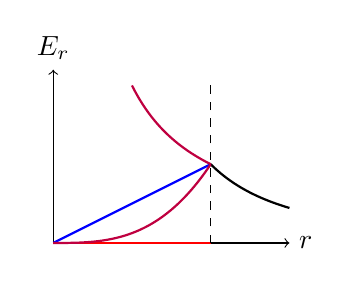
\begin{tikzpicture}
  \draw[->] (0, 0) -- (3, 0) node[right] {$r$};
  \draw[->] (0, 0) -- (0, 2.2) node[above] {$E_r$};
  \draw[thick, scale=1.0, domain=2:3, smooth, variable=\x, black] plot ({\x}, {4/(\x*\x)});
  \draw[thick, scale=1.0, domain=0:2, smooth, variable=\x, red] plot ({\x}, {0});
  \draw[thick, scale=1.0, domain=0:2, smooth, variable=\x, blue] plot ({\x}, {0.5*\x});
  \draw[thick, scale=1.0, domain=0:2, smooth, variable=\x, purple] plot ({\x}, {0.125*\x*\x*\x});
  \draw[thick, scale=1.0, domain=1:2, smooth, variable=\x, purple] plot ({\x}, {2/(\x)});
  \draw[dashed] (2,0) -- (2,2);
\end{tikzpicture}
\caption{Jackson problem (1.4)}
\end{figure}



\subsection{Exercise 1.5 Charge density of hydrogen atom}
With the potential
\begin{align}
\Phi=\frac{q}{4\pi\epsilon_0}\frac{e^{-\alpha r}}{r}\left(1+\frac{\alpha r}{2}\right)
\end{align}
we calculate for $r>0$
\begin{align}
\rho_1
&=-\epsilon_0\triangle\Phi\\
&=-\epsilon_0\frac{1}{r^2}\partial_r(r^2\partial_r\Phi)\\
&=-\frac{q}{4\pi}e^{-\alpha r}\frac{\alpha^3}{2}\\
&=-\frac{q}{\pi a_0^3}e^{-2r/a_0}
\end{align}
For $r=0$ we have
\begin{align}
\Phi(r\rightarrow0)&=\frac{q}{4\pi\epsilon_0r}\\
&\rightarrow\quad \rho_0=q\delta(r)
\end{align}
Therefore
\begin{align}
\rho&=\rho_0+\rho_1\\
&=q\left(\delta^{(3)}(r)-\frac{1}{\pi a_0^3}e^{-2r/a_0}\right)
\end{align}
Calculating the total charge
\begin{align}
Q_0&=q\int d^3r\delta(r)=q\\
Q_1
&=4\pi\int_0^\infty r^2\rho_1 dr\\
&=-\frac{4\pi q}{\pi a_0^3}\int_0^\infty r^2e^{-2r/a_0}dr\\
&=-\frac{4\pi q}{\pi a_0^3}\frac{a_0^3}{8}\int_0^\infty z^2e^{-z}dz\\
&=-\frac{4\pi q}{\pi a_0^3}\frac{a_0^3}{8}\Gamma(3)\\
&=-q
\end{align}

\subsection{Exercise 1.6 Simple capacitors}
(a) Assuming only front and back surfaces contribute
\begin{align}
2E_xA&=\frac{Q}{\epsilon_0}\\
\rightarrow\quad E_x&=\frac{Q}{2\epsilon_0A}\\
\rightarrow\quad \phi&=-\frac{Q}{2\epsilon_0A}x\\
\rightarrow\quad \phi_\text{tot}(x)&=-\frac{Q}{2\epsilon_0A}x-\frac{-Q}{2\epsilon_0A}(d-x)\\
&=-\frac{Q}{2\epsilon_0A}(x-(d-x))\\
&=-\frac{Q}{2\epsilon_0A}(2x-d)\\
\rightarrow\quad C&=\frac{Q}{\Delta\phi}=\frac{Q}{-\frac{Q}{2\epsilon_0A}(-d-d)}\\
&=\epsilon_0\frac{A}{d}
\end{align}
(b) The outer sphere does not contribute to the total potential as it is field free
\begin{align}
4\pi r^2 E_r&=\frac{Q}{\epsilon_0}\\
\rightarrow\quad E_r&=\frac{Q}{4\pi\epsilon_0 r^2}\\
\rightarrow\quad \phi&=\frac{Q}{4\pi\epsilon_0 r}\\
\rightarrow\quad \phi_\text{tot}&=\frac{Q}{4\pi\epsilon_0 r}\quad(a<r<b)\\
\rightarrow\quad C&=\frac{Q}{\Delta\phi}=\frac{Q}{\frac{Q}{4\pi\epsilon_0 b}-\frac{Q}{4\pi\epsilon_0 a}}\\
&=\epsilon_0\frac{4\pi ab}{b-a}
\end{align}
(c) 
\begin{align}
2\pi r L E_r=\frac{Q}{\epsilon_0}\\
\rightarrow\quad E_r&=\frac{Q}{2\pi r L\epsilon_0}\\
\rightarrow\quad \phi&=-\frac{Q}{2\pi L\epsilon_0}\log r\\
\rightarrow\quad \phi_\text{tot}&=-\frac{Q}{2\pi L\epsilon_0}\log r\quad(a<r<b)\\
\rightarrow\quad C&=\frac{Q}{\Delta\phi}=\frac{Q}{-\frac{Q}{2\pi L\epsilon_0}\log b+\frac{Q}{2\pi L\epsilon_0}\log a}\\
&=\frac{2\pi L\epsilon_0}{\log a/b}
\end{align}
(d) ...

\subsection{Exercise 1.7 Capacity of two parallel cylinders}Gauss law for one cylinder
\begin{align}
\oint_S\vec{E}\cdot\vec{n}dA&=\frac{1}{\epsilon_0}\int_V\rho(x)d^3x\\
2\pi rLE_r&=\frac{\rho_{1} L}{\epsilon_0}\\
E_r&=\frac{\rho}{2\pi\epsilon_0r}\\
\phi&=-\frac{\rho}{2\pi\epsilon_0}\ln r
\end{align}
For $d\gg a_{1,2}$ the potential of one cylinder on the surface of the second cylinder is constant - which means that the potential can be approximated by the sum of the potential of both cylinders (no need to make it complicated)
\begin{align}
\phi(\vec{r})&=\phi_1+\phi_2\\
&=-\frac{\rho_{1}}{2\pi\epsilon_0}\ln |\vec{r}|-\frac{\rho_{2}}{2\pi\epsilon_0}\ln |\vec{r}-\vec{d}|\\
&=-\frac{\rho}{2\pi\epsilon_0}\ln |\vec{r}|+\frac{\rho}{2\pi\epsilon_0}\ln |\vec{r}-\vec{d}|\\
&=-\frac{\rho}{2\pi\epsilon_0}\left(\ln |\vec{r}|-\ln |\vec{r}-\vec{d}|\right)\\
&=-\frac{\rho}{2\pi\epsilon_0}\ln \frac{|\vec{r}|}{|\vec{r}-\vec{d}|}\\
&=-\frac{\rho}{\pi\epsilon_0}\ln \sqrt{\frac{|\vec{r}|}{|\vec{r}-\vec{d}|}}
\end{align}
Then the potential difference between to surfaces is given by (with $\vec{n}=\vec{d}/d$ and $\rho=\rho_1=-\rho_2$)
\begin{align}
\Delta\phi&=\phi(a_1\vec{n})-\phi((d-a_2)\vec{n})\\
&=-\frac{\rho}{\pi\epsilon_0}\left(\ln \sqrt{\frac{a_1}{d-a_1}}-\ln \sqrt{\frac{d-a_2}{a_2}}\right)\\
&=\frac{\rho}{\pi\epsilon_0}\left(\ln \sqrt{\frac{d-a_1}{a_1}}+\ln \sqrt{\frac{d-a_2}{a_2}}\right)\\
&\simeq\frac{\rho}{\pi\epsilon_0}\left(\ln \sqrt{\frac{d}{a_1}}+\ln \sqrt{\frac{d}{a_2}}\right)\\
&\simeq\frac{\rho}{\pi\epsilon_0}\ln \frac{d}{\sqrt{a_1a_2}}
\end{align}
With $C=Q/U$ we have
\begin{align}
C=\frac{\rho L}{\Delta\phi}&=\frac{\pi\epsilon_0L}{\ln \frac{d}{\sqrt{a_1a_2}}}
\end{align}
which is the desired result. The numbers are 0.49mm, 1.47mm and 4.92mm.


\subsection{Exercise 1.8 Energy of capacitors}
\begin{align}
W
=\frac{1}{2}\int\rho(x)\phi(x)d^3x
=-\frac{\epsilon_0}{2}\int\phi\triangle\phi d^3x
=\frac{\epsilon_0}{2}\int(\nabla\phi)^2 d^3x
=\frac{\epsilon_0}{2}\int|\vec{E}|^2 d^3x
\end{align}
(a) With $\vec{E}_\text{tot}=-\nabla\phi_\text{tot}$ and $Q=C\cdot U$
\begin{align}
W_\text{plate}&=\frac{\epsilon_0}{2}\cdot\left(\frac{Q}{\epsilon_0A}\right)^2\cdot(Ad)=\frac{Q^2d}{2\epsilon_0A}\\
&=\frac{U^2d}{2\epsilon_0A}\left(\frac{\epsilon_0A}{d}\right)^2=
\frac{\epsilon_0AU^2}{2d}
\end{align}
\begin{align}
W_\text{sphere}&=\frac{\epsilon_0}{2}4\pi\int_a^br^2\frac{Q^2}{16\pi^2\epsilon_0^2r^4}dr=\frac{Q^2}{8\pi\epsilon_0}\left(\frac{1}{b}-\frac{1}{a}\right)\\
&=\frac{U^2}{8\pi\epsilon_0}\left(\frac{a-b}{ab}\right)\cdot\left(\epsilon_0\frac{4\pi ab}{b-a}\right)^2=2\pi\epsilon_0U^2\frac{ab}{b-a}
\end{align}
\begin{align}
W_\text{cylinder}&=\frac{\epsilon_0}{2}2\pi L\int_a^b\left(\frac{Q}{2\pi\epsilon_0Lr}\right)^2r\;dr
=\frac{Q^2}{4\pi\epsilon_0L}\log\frac{b}{a}\\
&=\frac{U^2}{4\pi\epsilon_0L}\log\frac{b}{a}\left(\frac{2\pi\epsilon_0 L}{\log b/a}\right)^2=\frac{\pi\epsilon_0LU^2}{\log b/a}
\end{align}
(b) 
\begin{align}
w_\text{plate}&=\text{const}\\
w_\text{sphere}&\sim r^{-4}\\
w_\text{cylinder}&\sim r^{-2}
\end{align}

\subsection{Exercise 5.1 Biot–Savart law NOT DONE YET}
With
\begin{align}
\nabla_{x'}\frac{1}{|\mathbf{x}-\mathbf{x'}|}
=\frac{\mathbf{x}-\mathbf{x'}}{|\mathbf{x}-\mathbf{x'}|^3}
\end{align}
we consider a loop of radius $a$ in the $x-y$ plane
\begin{align}
d\mathbf{B}&=\frac{\mu_0I}{4\pi}d\mathbf{l}'\times\frac{\mathbf{x}-\mathbf{x'}}{|\mathbf{x}-\mathbf{x'}|^3}\\
\mathbf{B}(\mathbf{x})
&=\frac{\mu_0I}{4\pi}\oint_{C}d\mathbf{l}'\times\frac{\mathbf{x}-\mathbf{x'}}{|\mathbf{x}-\mathbf{x'}|^3}\\
&=\frac{\mu_0I}{4\pi}\oint_{C}d\mathbf{l}'\times\left(\nabla_{x'}\frac{1}{|\mathbf{x}-\mathbf{x'}|}\right)
\end{align}
with $P$ in the $x-z$ plane
\begin{align}
(\mathbf{x}-\mathbf{x'})^2
&=(r\cos\theta)^2+((r\sin\theta)^2+a^2-2ar\sin\theta\cos\phi')\\
&=r^2+a^2-2ar\sin\theta\cos\phi'
\end{align}

\subsection{Exercise 9.1 Rotating charge and current densities - NOT DONE YET}
With $r=|\mathbf{x}|$ and $r'=|\mathbf{x}'|$
\begin{align}
\mathbf{A}(\mathbf{x},t)&=\frac{\mu_0}{4\pi}\int dt'\int d^3\mathbf{x}'\frac{\mathbf{J}(\mathbf{x}',t')}{|\mathbf{x}-\mathbf{x}'|}\delta\left(t'+\frac{|\mathbf{x}-\mathbf{x}'|}{c}-t\right)\\
&=\frac{\mu_0}{4\pi}\int dt'\int d^3\mathbf{x}'\frac{\mathbf{J}(\mathbf{x}',t-|\mathbf{x}-\mathbf{x}'|/c)}{|\mathbf{x}-\mathbf{x}'|}\\
&=\frac{\mu_0}{4\pi}\sum_{l,m}\frac{4\pi}{2l+1}\frac{q_{lm}}{r^{l+1}}Y_{lm}(\vartheta,\varphi)\\
q_{lm}(t)&=\int d^3\mathbf{x}'\,r'^l\,Y_{lm}^*(\vartheta',\varphi')\,\mathbf{J}(\mathbf{x}',t-|\mathbf{x}-\mathbf{x}'|/c)\\
\mathbf{J}(\mathbf{x}',t)&=\rho(\mathbf{x}',t)\mathbf{v}
=(\mathbf{\Omega}\times\mathbf{x'})\rho(\mathbf{x}',t)
\end{align}

\subsection{Exercise 9.2 Rotating quadrupole - NOT DONE YET}
Lets look at a single rotating point charge first
\begin{align}
\rho(\mathbf{x}',t')
&=\frac{1}{r'^2\sin\theta'}q\delta(r'-R)\delta(\phi'-\omega t')\delta(\theta'-\pi/2)\\
\mathbf{J}(\mathbf{x}',t')
&=\rho\mathbf{v}\\
&=\frac{1}{r'^2\sin\theta'}q\delta(r'-R)\delta(\phi'-\omega t')\delta(\theta'-\pi/2)R\omega\mathbf{e}_\phi
\end{align}

\begin{eqnarray}
Y_{00}=\frac{1}{\sqrt{4\pi}} 
&Y_{10}=\sqrt{\frac{3}{4\pi}}\cos\theta
&Y_{20}=\sqrt{\frac{5}{16\pi}}(3\cos^2\theta-1)\\
%
Y_{11}=-\sqrt{\frac{3}{8\pi}}\sin\theta\,e^{i\phi}
&Y_{1,-1}=\sqrt{\frac{3}{8\pi}}\sin\theta\,e^{-i\phi}
&Y_{21}=-\sqrt{\frac{15}{8\pi}}\sin\theta\cos\theta\,e^{i\phi}\\
%
Y_{2,-1}=\sqrt{\frac{15}{8\pi}}\sin\theta\cos\theta\,e^{-i\phi}
&Y_{22}=\sqrt{\frac{15}{32\pi}}\sin^2\theta\,e^{2i\phi}
&Y_{2,-2}=\sqrt{\frac{15}{32\pi}}\sin^2\theta\,e^{-2i\phi}
\end{eqnarray}



\begin{align}
\rho(\mathbf{x},t)
&=q\delta\left(x-\frac{a}{\sqrt{2}}\cos\omega t\right)\delta\left(y-\frac{a}{\sqrt{2}}\sin\omega t\right)\delta(z)
+q\delta\left(x+\frac{a}{\sqrt{2}}\cos\omega t\right)\delta\left(y+\frac{a}{\sqrt{2}}\sin\omega t\right)\delta(z)\\
&-q\delta\left(x+\frac{a}{\sqrt{2}}\sin\omega t\right)\delta\left(y-\frac{a}{\sqrt{2}}\cos\omega t\right)\delta(z)
-q\delta\left(x-\frac{a}{\sqrt{2}}\sin\omega t\right)\delta\left(y+\frac{a}{\sqrt{2}}\cos\omega t\right)\delta(z)\\
\end{align}

\subsection{Exercise 12.1 Lagrangian of point charge}
\begin{enumerate}
\item With $U^\alpha=\frac{dx_\alpha}{ds}$
\begin{align}
	L&=-\frac{mU_\alpha U^\alpha}{2}-\frac{q}{c}U_\alpha A^\alpha\\
	\frac{\partial L}{\partial x_\beta}&=-\frac{q}{c}U_\alpha\frac{\partial A^\alpha}{\partial x_\beta}\\
	\frac{\partial L}{\partial U_\beta}&=-mU^\beta-\frac{q}{c}A^\beta
\end{align}
\begin{align}
	-m\frac{d}{ds}\left(\frac{dU^\beta}{ds}\right)-\frac{q}{c}\frac{dA^\beta}{ds}+\frac{q}{c}U_\alpha\frac{\partial A^\alpha}{\partial x_\beta}=0\\
	m\frac{d^2x^\beta}{ds^2}+\frac{q}{c}\frac{dA^\beta}{ds}-\frac{q}{c}\frac{dx_\alpha}{ds}\frac{\partial A^\alpha}{\partial x_\beta}=0\\
	m\frac{d^2x^\beta}{ds^2}+\frac{q}{c}\left(\frac{\partial A^\beta}{\partial x^\alpha}\frac{\partial x^\alpha}{\partial s}\right)-\frac{q}{c}\frac{dx_\alpha}{ds}\frac{\partial A^\alpha}{\partial x_\beta}=0\\
	m\frac{d^2x^\beta}{ds^2}+\frac{q}{c}\frac{\partial x^\alpha}{\partial s}\left(\frac{\partial A^\beta}{\partial x^\alpha}-\frac{\partial A^\alpha}{\partial x_\beta}\right)=0\\
	m\frac{d^2x^\beta}{ds^2}+\frac{q}{c}\frac{\partial x^\alpha}{\partial s}F^{\alpha\beta}=0
\end{align}
\item Bit of a odd sign convention for the canonical momentum
\begin{align}
P^\beta&=-\frac{\partial L}{\partial U_\beta}=mU^\beta+\frac{q}{c}A^\beta\quad\rightarrow\quad U^\beta=\frac{1}{m}\left(P^\beta-\frac{q}{c}A^\beta\right)\\
H&=P^\alpha U_\alpha+L\\
&=P^\alpha\frac{1}{m}\left(P_\alpha-\frac{q}{c}A_\alpha\right)-\frac{m}{2}\frac{1}{m}\left(P_\alpha-\frac{q}{c}A_\alpha\right)\frac{1}{m}\left(P_\alpha-\frac{q}{c}A_\alpha\right)-\frac{q}{c}\frac{1}{m}\left(P_\alpha-\frac{q}{c}A_\alpha\right)A^\alpha\\
&=\frac{1}{2m}\left(P^\alpha-\frac{q}{c}A^\alpha\right)\left(P_\alpha-\frac{q}{c}A_\alpha\right)
\end{align}
In space-time coordinates we can write
\begin{align}
H&=\frac{1}{2m}\left((p_0)^2-\vec{p}^2+\frac{q^2}{c^2}[\phi^2-\vec{A}^2]+\frac{2q}{c}[\vec{p}\cdot\vec{A}-p^0\phi]\right)\\
&=\frac{1}{2m}\left((\gamma m c)^2-(\gamma m\vec{v})^2+\frac{q^2}{c^2}[\phi^2-\vec{A}^2]+\frac{2q}{c}[\gamma m\vec{v}\cdot\vec{A}-\gamma m c\phi]\right)\\
&=\frac{\gamma^2mc^2}{2}\left(1-\frac{\vec{v}^2}{c^2}\right)+\frac{q^2}{2mc^2}[\phi^2-\vec{A}^2]+q\gamma[\frac{1}{c}\vec{v}\cdot\vec{A}- \phi]\\
&=\frac{mc^2}{2}+\frac{q^2}{2mc^2}[\phi^2-\vec{A}^2]+q\gamma[\frac{1}{c}\vec{v}\cdot\vec{A}- \phi]
\end{align}
\end{enumerate}

\section{{\sc Schwinger} - Classical Electrodynamics}
\subsection{Exercise 9.1 Lagrangian of a particle in an electromagnetic field}
\begin{align}
L=\mathbf{p}\cdot\left(\frac{d\mathbf{r}}{dt}-\mathbf{v}\right)+\frac{1}{2}mv^2-e\phi+\frac{e}{c}\mathbf{v}\cdot\mathbf{A}
\end{align}


\subsection{Exercise 31.1 Potentials of moving point charge}
\begin{align}
    w=z-vt
    \rightarrow
    \frac{\partial}{\partial z}&=\frac{\partial w}{\partial z}\frac{\partial}{\partial w}\\
    \rightarrow\frac{\partial^2}{\partial z^2}&=\frac{\partial^2 w}{\partial z^2}\frac{\partial}{\partial w}+\left(\frac{\partial w}{\partial z}\right)^2\frac{\partial^2}{\partial w^2}=\frac{\partial^2}{\partial w^2}\\
    \rightarrow\frac{\partial^2}{\partial t^2}&=\frac{\partial^2 w}{\partial t^2}\frac{\partial}{\partial w}+\left(\frac{\partial w}{\partial t}\right)^2\frac{\partial^2}{\partial w^2}=v^2\frac{\partial^2}{\partial w^2}
\end{align}
then
\begin{align}
    \triangle-\frac{1}{c^2}\frac{\partial^2}{\partial t^2}&=\frac{\partial^2}{\partial x^2}+\frac{\partial^2}{\partial y^2}+\frac{\partial^2}{\partial w^2}-\frac{v^2}{c^2}\frac{\partial^2}{\partial w^2}\\
    &=\frac{\partial^2}{\partial x^2}+\frac{\partial^2}{\partial y^2}+\left(1-\frac{v^2}{c^2}\right)\frac{\partial^2}{\partial w^2}\\
    &=\frac{\partial^2}{\partial x^2}+\frac{\partial^2}{\partial y^2}+\frac{\partial^2}{\partial u^2}
\end{align}
with with $u=w/\sqrt{1-v^2/c^2}$. The wave equation can then be rewritten
\begin{align}
    -\Box\phi&=4\pi\rho\\
    &=4\pi e\delta(x)\delta(y)\delta(z-vt)\\
    -\left(\frac{\partial^2}{\partial x^2}+\frac{\partial^2}{\partial y^2}+\frac{\partial^2}{\partial u^2}\right)\phi&=4\pi e\delta(x)\delta(y)\delta\left(\sqrt{1-\frac{v^2}{c^2}}u\right)\\
    &=\frac{4\pi}{\sqrt{1-\frac{v^2}{c^2}}} e\delta(x)\delta(y)\delta\left(u\right)
\end{align}
Using the Green function of the Coulomb equation (13.3) we obtain
\begin{align}
    \phi&=\frac{e}{\sqrt{1-\frac{v^2}{c^2}}\sqrt{u^2+x^2+y^2}}\\
    &=\frac{e}{\sqrt{w^2+(1-\frac{v^2}{c^2})(x^2+y^2})}\\
    &=\frac{e}{\sqrt{(z-vt)^2+(1-\frac{v^2}{c^2})(x^2+y^2})}
\end{align}
For the vector potential we can calculate similarly
\begin{align}
    -\Box\vec{A}&=4\pi\frac{\vec{j}}{c}\\
    -\left(\frac{\partial^2}{\partial x^2}+\frac{\partial^2}{\partial y^2}+\frac{\partial^2}{\partial u^2}\right)\vec{A}&=4\pi e\frac{\vec{v}}{c}\delta(x)\delta(y)\delta\left(\sqrt{1-\frac{v^2}{c^2}}u\right)\\
    &=\frac{4\pi}{\sqrt{1-\frac{v^2}{c^2}}} e\frac{\vec{v}}{c}\delta(x)\delta(y)\delta\left(u\right)
\end{align}
which gives $\vec{A}=\vec{v}/c\phi$.

\subsection{Exercise 31.2 Fields of moving point charge}
\begin{align}
	\vec{E}&=-\nabla\phi-\frac{1}{c}\frac{\partial\vec{A}}{\partial t}\\
	&=\frac{e}{2}\left((z-vt)^2+(1-\frac{v^2}{c^2})(x^2+y^2)\right)^{-3/2}[(1-\frac{v^2}{c^2})2x,(1-\frac{v^2}{c^2})2y,2(z-vt)(1-\frac{v^2}{c^2})]\\
	&=e(1-\frac{v^2}{c^2})\left((z-vt)^2+(1-\frac{v^2}{c^2})(x^2+y^2)\right)^{-3/2}[x,y,(z-vt)]\\
	\vec{B}&=\nabla\times\vec{A}\\
	&=-e\frac{v}{c}(1-\frac{v^2}{c^2})\left((z-vt)^2+(1-\frac{v^2}{c^2})(x^2+y^2)\right)^{-3/2}[y,x,0]
\end{align}

\subsection{Exercise 31.4 Wave equation for fields}
With
\begin{align}
\nabla\times\vec{B}&=\frac{1}{c}\frac{\partial}{\partial t}\vec{E}+\frac{4\pi}{c}\vec{j}_e\\
\nabla\cdot\vec{E}&=4\pi\rho_e\\
-\nabla\times\vec{E}&=\frac{1}{c}\frac{\partial}{\partial t}\vec{B}+\frac{4\pi}{c}\vec{j}_m\\
\nabla\cdot\vec{B}&=4\pi\rho_m
\end{align}
we obtain
\begin{align}
\nabla\times\nabla\times\vec{B}
&=\nabla(\nabla\cdot\vec{B})-\triangle\vec{B}\\
&=4\pi\nabla\rho_m-\triangle\vec{B}\\
&=\frac{1}{c}\frac{\partial}{\partial t}\nabla\times\vec{E}+\frac{4\pi}{c}\nabla\times\vec{j}_e\\
&=-\frac{1}{c^2}\frac{\partial^2}{\partial t^2}\vec{B}-\frac{4\pi}{c^2}\frac{\partial}{\partial t}\vec{j}_m+\frac{4\pi}{c}\nabla\times\vec{j}_e\\
&\rightarrow-\Box\vec{B}=-4\pi\nabla\rho_m+\frac{4\pi}{c}(\nabla\times\vec{j}_e-\frac{1}{c}\frac{\partial}{\partial t}\vec{j}_m)
\end{align}

\begin{align}
\nabla\times\nabla\times\vec{E}
&=\nabla(\nabla\cdot\vec{E})-\triangle\vec{E}\\
&=4\pi\nabla\rho_e-\triangle\vec{E}\\
&=-\frac{1}{c}\frac{\partial}{\partial t}\nabla\times\vec{B}-\frac{4\pi}{c}\nabla\times\vec{j}_m\\
&=-\frac{1}{c^2}\frac{\partial^2}{\partial t^2}\vec{E}-\frac{4\pi}{c^2}\frac{\partial}{\partial t}\vec{j}_e-\frac{4\pi}{c}\nabla\times\vec{j}_m\\
&\rightarrow-\Box\vec{E}=-4\pi\nabla\rho_e+\frac{4\pi}{c}(\nabla\times\vec{j}_m-\frac{1}{c}\frac{\partial}{\partial t}\vec{j}_e)
\end{align}

\subsection{Exercise 31.5 Lienard-Wiechert potentials}
We start with the scalar potential
\begin{align}
\phi(\mathbf{r},t)&=\int d\vec{r}'dt'\frac{\delta(\frac{1}{c}|\mathbf{r}-\mathbf{r}'|-(t-t'))}{|\mathbf{r}-\mathbf{r}'|}\rho(\mathbf{r}',t')\\
&=\int d\mathbf{r}'dt'\frac{\delta(t'-t+\frac{1}{c}|\mathbf{r}-\mathbf{r}'|)}{|\mathbf{r}-\mathbf{r}'|}e\delta(\mathbf{r}'-\mathbf{r}_B(t'))\\
&=\int dt'\frac{e}{|\mathbf{r}-\mathbf{r}_B(t')|}\delta(t'-t+\frac{1}{c}|\mathbf{r}-\mathbf{r}_B(t')|)
\end{align}
with
\begin{align}
\delta(t'-t+\frac{1}{c}|\mathbf{r}-\mathbf{r}_B(t')|)&=\delta(f(t'))\\
&=\sum_{t_{ret}}\frac{\delta(t'-t_{ret})}{|f'(t_{ret})|}
\end{align}
where
\begin{align}
f(t')&=t'-t+\frac{1}{c}|\mathbf{r}-\mathbf{r}'_B(t')|\\
f(t_{ret})&=t_{ret}-t+\frac{1}{c}|\mathbf{r}-\mathbf{r}_B(t_{ret})|=0\\
\rightarrow t_{ret}&=t-\frac{1}{c}|\mathbf{r}-\mathbf{r}_B(t_{ret})|\\
f'(t')&=1+\frac{1}{c}\partial_{t'}|\mathbf{r}-\mathbf{r}_B(t')|\\
&=1+\frac{1}{c}\frac{2\mathbf{r}_{B}\cdot\mathbf{v}_{B}(t')-2\mathbf{r}\cdot\mathbf{v}_{B}(t')}{2|\mathbf{r}-\mathbf{r}'_B(t')|}\\
&\qquad\qquad\qquad\text{using}\quad|\mathbf{r}-\mathbf{r}_B(t')|=\sqrt{r^2+r_B^2-2\mathbf{r}\cdot\mathbf{r}_B}\\
&=1+\frac{1}{c}\frac{(\mathbf{r}_{B}(t')-\mathbf{r})\cdot\mathbf{v}_{B}(t')}{|\mathbf{r}-\mathbf{r}_B(t')|}
\end{align}
then
\begin{align}
\delta(t'-t+\frac{1}{c}|\mathbf{r}-\mathbf{r}_B(t')|)
&=\frac{\delta(t'-t_{ret})}{|f'(t_{ret})|}\\
&=\frac{\delta(t'-t_{ret})}{1+\frac{1}{c}\frac{(\mathbf{r}_{B}(t_{ret})-\mathbf{r})\cdot\mathbf{v}_{B}(t_{ret})}{|\mathbf{r}-\mathbf{r}_B(t_{ret})|}}
\end{align}
and therefore
\begin{align}
\phi(\mathbf{r},t)
&=\int dt'\frac{e}{|\mathbf{r}-\mathbf{r}_B(t')|}\delta(t'-t+\frac{1}{c}|\mathbf{r}-\mathbf{r}_B(t')|)\\
&=\int dt'\frac{e}{|\mathbf{r}-\mathbf{r}_B(t')|}\frac{\delta(t'-t_{ret})}{1+\frac{1}{c}\frac{(\mathbf{r}_{B}(t_{ret})-\mathbf{r})\cdot\mathbf{v}_{B}(t_{ret})}{|\mathbf{r}-\mathbf{r}_B(t_{ret})|}}\\
&=\frac{e}{|\mathbf{r}-\mathbf{r}_B(t_{ret})|+\frac{1}{c}(\mathbf{r}_{B}(t_{ret})-\mathbf{r})\cdot\mathbf{v}_{B}(t_{ret})}\\
&=\frac{e}{|\mathbf{r}-\mathbf{r}_B(t_{ret})|-[\mathbf{r}-\mathbf{r}_{B}(t_{ret})]\cdot\frac{\mathbf{v}_{B}(t_{ret})}{c}}
\end{align}
Now let's look at the vector potential
\begin{align}
\mathbf{A}(\mathbf{r},t)
&=\frac{1}{c}\int d\vec{r}'dt'\frac{\delta(\frac{1}{c}|\mathbf{r}-\mathbf{r}'|-(t-t'))}{|\mathbf{r}-\mathbf{r}'|}\mathbf{j}(\mathbf{r}',t')\\
&=\frac{e}{c}\int d\vec{r}'dt'\frac{\delta(\frac{1}{c}|\mathbf{r}-\mathbf{r}'|-(t-t'))}{|\mathbf{r}-\mathbf{r}'|}\mathbf{v}(t')\delta(\mathbf{r}'-\mathbf{r}_B(t'))\\
&=\frac{e}{c}\int dt'\frac{\delta(\frac{1}{c}|\mathbf{r}-\mathbf{r}_B(t')|-(t-t'))}{|\mathbf{r}-\mathbf{r}_B(t')|}\mathbf{v}(t')\\
&=...\\
&=\frac{\mathbf{v}_B(t')}{c}\phi(\mathbf{r},t)
\end{align}




\subsection{Exercise 38.1 Total radiated power}
We observe
\begin{align}
\frac{\lambda}{(1+\lambda\beta)^4}=-\frac{1}{\beta(1+\lambda\beta)^4}+\frac{1}{\beta(1+\lambda\beta)^3}.    
\end{align}
Then
\begin{align}
    f(\lambda)&=\frac{2}{(1+\lambda\beta)^3}\left(-\frac{\beta^2}{2}+\frac{\lambda\beta}{8}\frac{\beta^2-1}{1+\lambda\beta}\right)\\
    &=-\beta^2\frac{1}{(1+\lambda\beta)^3}+\frac{\beta(\beta^2-1)}{4}\frac{\lambda}{(1+\lambda\beta)^4}\\
    &=\left(-\beta^2+\frac{\beta^2-1}{4}\right)\frac{1}{(1+\lambda\beta)^3}-\frac{(\beta^2-1)}{4}\frac{1}{(1+\lambda\beta)^4}\\
    \int_{-1}^1f(\lambda)d\lambda&=-\frac{1+3\lambda^2}{4}
\end{align}

\section{{\sc Wald} - Advanced Classical Electrodynamics}

\subsection{Problem 2.3 The proton and the hydrogen atom}
\begin{enumerate}[(a)]
\item Using Gauss law with spherical symmetry inside the nucleus
\begin{align}
4\pi r^2 E_r(r)&=\frac{1}{\varepsilon_0}\frac{4}{3}\pi r^3\rho\\
4\pi R^2 E_r(r)&=\frac{1}{\varepsilon_0}\frac{4}{3}\pi R^3\rho=\frac{Q}{\varepsilon_0}\quad\rightarrow\quad\rho=\frac{Q}{\frac{4}{3}\pi R^3}\\
E_r(r)&=\frac{1}{\varepsilon_0}\frac{Qr}{4\pi R^3}
\end{align}
and outside
\begin{align}
E_r(r)&=\frac{1}{\varepsilon_0}\frac{Q}{4\pi r^2}
\end{align}
Then the field energy is
\begin{align}
\mathscr{E}
&=\frac{\varepsilon_0}{2}4\pi\left[\left(\frac{Q}{4\pi\varepsilon_0 R^3}\right)^2\int_0^Rr^2r^2\;dr+\left(\frac{Q}{4\pi\varepsilon_0}\right)^2\int_0^Rr^2\frac{1}{r^4}\;dr\right]\\
&=\frac{3Q^2}{20\pi\varepsilon_0 R}\\
&=1.4\cdot 10^{-13}\text{J}\\
&=0.87\text{MeV}
\end{align}
while $mc^2=939$MeV.
\item Interaction energy - we assume the proton to be a point charge
\begin{align}
\mathscr{E}
&=\varepsilon_0\int d^3x\; \mathbf{E}_\text{proton}\cdot\mathbf{E}_\text{1s}\\
&=\varepsilon_0\int d^3x\; E_\text{proton,r}\cdot E_\text{1s,r}\\
&\simeq4\pi\varepsilon_0\int_0^\infty dr r^2\frac{1}{\varepsilon_0}\frac{Q}{4\pi r^2}\cdot\frac{-Q e^{-2r/a}}{\pi a^3}\\
&\simeq-\frac{Q^2}{\pi a^3}\int_0^\infty dr e^{-2r/a}\\
&\simeq\frac{Q^2}{\pi a^3}\frac{a}{2} \left[e^{-2r/a}\right]^\infty_0\\
&\simeq-\frac{Q^2}{\pi a^3}\frac{a}{2}=-\frac{Q^2}{2\pi a^2}\\
&\simeq-9.1\text{eV}
\end{align}
with $\langle T\rangle=\frac{1}{2}\langle V\rangle$ we get to 13.6eV.
\end{enumerate}


\subsection{Problem 2.4 Potential from oddly shaped charge distribution}
We need to calculate
\begin{align}
\phi(\vec{r})=\frac{1}{4\pi\varepsilon_0}\int\frac{\rho(r')}{|\vec{r}-\vec{r}'|}d^3\vec{r}'
\end{align}
trying to avoid the brute force calculation we see that we can expand the charge distribution in a finite series of Legendre polynomials
\begin{align}
(1-\cos\theta)^2=\frac{4}{3}P_0(\cos\theta)-2P_1(\cos\theta)+\frac{2}{3}P_2(\cos\theta)
\end{align}
where we used the orthogonality of the Legendre polynomials to project out the coefficients 
\begin{align}
\int_{-1}^{+1}P_n(x)P_m(x)dx&=\frac{2}{2n+1}\delta_{mn}\\
\int_{0}^{\pi}P_n(\cos\theta)P_m(\cos\theta)\sin\theta\,d\theta&=\frac{2}{2n+1}\delta_{mn}
\end{align}
with the multipole expansion ({\bf for the outside})
\begin{align}
\frac{1}{|\vec{r}-\vec{r}'|}
&=\frac{1}{\sqrt{r^2+r'^2-2rr'\cos\theta}}\\
&=\frac{1}{r\sqrt{1+\frac{r'^2}{r^2}-2\frac{r'}{r}\cos\theta}}\\
&=\frac{1}{r}\sum_lP_l(\cos\theta)\frac{r'^l}{r^l}
\end{align}
we can insert all into the Coulomb integral and utilize the orthogonality of the Legendre polynomials again
\begin{align}
\phi(\vec{r})
&=\frac{2\pi\alpha}{4\pi\varepsilon_0r}\int_0^R dr'r'^2(R-r')\sum_l\frac{r'^l}{r^l}\int d\theta P_l(\cos\theta)\left(\frac{4}{3}P_0(\cos\theta)-2P_1(\cos\theta)+\frac{2}{3}P_2(\cos\theta)\right)\sin\theta\\
&=\frac{\alpha}{2\varepsilon_0r}\int_0^R dr'r'^2\frac{r'^l}{r^l}(R-r')\left[\frac{4}{3}\frac{2}{2\cdot0+1}-2\frac{2}{2\cdot1+1}\frac{r'}{r}+\frac{2}{3}\frac{2}{2\cdot2+1}\frac{r'^2}{r^2}\right]\\
&=...\\
&=\frac{\alpha R^4}{9r\varepsilon_0}\left(1-\frac{3R}{10r}+\frac{R^2}{25r^2}\right)
\end{align}

\subsection{Exercise 5.1}
Vacuum equations
\begin{align}
\nabla\cdot\mathbf{E}&=\frac{\rho}{\epsilon_0}\qquad\nabla\times\mathbf{B}=\mu_0\mathbf{J}+\frac{1}{c^2}\frac{\partial\mathbf{E}}{\partial t}\\
\nabla\cdot\mathbf{B}&=0\qquad\nabla\times\mathbf{E}=-\frac{\partial\mathbf{B}}{\partial t}
\end{align}
then
\begin{align}
\nabla\times(\nabla\times\mathbf{E})&=-\frac{\partial}{\partial t}\nabla\times\mathbf{B}\\
\nabla(\nabla\cdot\mathbf{E})-\triangle^2\mathbf{E}&=-\mu_0\frac{\partial\mathbf{J}}{\partial t}-\frac{1}{c^2}\frac{\partial^2\mathbf{E}}{\partial t^2}\\
\rightarrow\Box\mathbf{E}&=\mu_0\frac{\partial\mathbf{J}}{\partial t}+\frac{1}{\epsilon_0}\nabla\rho
\end{align}
\begin{align}
\nabla\times(\nabla\times\mathbf{B})&=\mu_0\nabla\times\mathbf{J}+\frac{1}{c^2}\frac{\partial}{\partial t}\nabla\times\mathbf{E}\\
\nabla(\nabla\cdot\mathbf{B})-\triangle^2\mathbf{B}&=\mu_0\nabla\times\mathbf{J}-\frac{1}{c^2}\frac{\partial^2\mathbf{B}}{\partial t^2}\\
\rightarrow\Box\mathbf{B}&=-\mu_0\nabla\times\mathbf{J}
\end{align}
Construction a solution:
Now observe that the charge continuity equation $\dot\rho+\nabla\cdot\mathbf{J}=0$ can not be recovered from the two equations.
So lets assume $\mathbf{J}=0$ and $\rho(t)=q(t)\delta(\mathbf{x})$ then we set
\begin{align}
\mathbf{B}&=0\\
\mathbf{E}&=\frac{1}{4\pi\epsilon_0}\frac{q(t)}{r^2}
\end{align}
which violates $\nabla\times\mathbf{B}$


\section{{\sc Smythe} - Static and Dynamic Electricity}
\subsection{Exercise 1.1 Two coaxial rings and a point charge}
Total charge of an axial ringlike charge distribution
\begin{align}
    Q&=\int \rho_0(\varphi')\delta(z'-0)\delta(r'-a) d\varphi' dz' dr'\\
    &=2\pi a\rho_0
\end{align}
which means that the 1-dimensional charge density is $\rho_0=Q/2\pi a$.
The axial potential of a single ring is then
\begin{align}
    \phi(z)&=\frac{1}{4\pi\varepsilon_0}\int\frac{\rho_0\delta(z'-0)\delta(r'-a)}{\sqrt{a^2+z^2}}r d\varphi' dz' dr'\\
    &=\frac{1}{4\pi\varepsilon_0}2\pi a \rho_0\frac{1}{\sqrt{a^2+z^2}}\\
    &=\frac{Q}{4\pi\varepsilon_0}\frac{1}{\sqrt{a^2+z^2}}
\end{align}
therefore we get for the energies
\begin{align}
    W_1&=\frac{qQ_1}{4\pi\varepsilon_0}\frac{1}{a}+\frac{qQ_2}{4\pi\varepsilon_0}\frac{1}{\sqrt{a^2+b^2}}\\
    W_2&=\frac{qQ_1}{4\pi\varepsilon_0}\frac{1}{\sqrt{a^2+b^2}}+\frac{qQ_2}{4\pi\varepsilon_0}\frac{1}{a}
\end{align}
solving the linear system for the charges $Q_{1,2}$ we obtain
\begin{align}
    Q_1&=\frac{4\pi\varepsilon_0}{qb^2}\sqrt{a^2+b^2}\left(\sqrt{a^2+b^2}W_1-aW_2\right)\\
    Q_2&=\frac{4\pi\varepsilon_0}{qb^2}\sqrt{a^2+b^2}\left(-aW_1+\sqrt{a^2+b^2}W_2\right).
\end{align}

\subsection{Exercise 1.3 Flux of two point charges through circle}
For the flux we have
\begin{align}
    N&\equiv\int\vec{E}\cdot d\vec{A}\\
    &=\int E \cos(\vec{E},\vec{n})\ dA\\
    &=2\pi\int\frac{q}{4\pi\varepsilon_0(a^2+r^2)}\frac{a}{\sqrt{a^2+r^2}}rdr-2\pi\int\frac{Q}{4\pi\varepsilon_0(a^2+r^2)}\frac{a}{\sqrt{a^2+r^2}}rdr\\
    &=\frac{2\pi a}{4\pi\varepsilon_0}(q-Q)\int_0^a\frac{1}{(a^2+r^2)^{3/2}}rdr\\
    &=\frac{1}{4\varepsilon_0}(q-Q)\left(2-\sqrt{2}\right)
\end{align}
therefore
\begin{align}
    Q=q-\frac{4N\varepsilon_0}{2-\sqrt{2}}.
\end{align}

\subsection{Exercise 1.4 Concentric charged rings}
The axial potential of a single ring is with radius $a$ and charge $Q=2\pi a\rho_0$ is
\begin{align}
    \phi(x)&=\frac{1}{4\pi\varepsilon_0}\int\frac{\rho_0\delta(z'-0)\delta(r'-a)}{\sqrt{a^2+x^2}}r d\varphi' dz' dr'\\
    &=\frac{1}{4\pi\varepsilon_0}2\pi a \rho_0\frac{1}{\sqrt{a^2+x^2}}\\
    &=\frac{Q}{4\pi\varepsilon_0}\frac{1}{\sqrt{a^2+x^2}}
\end{align}
The total potential and the resulting electrical field is therefore
\begin{align}
    \phi(x)&=-\frac{Q}{4\pi\varepsilon_0}\frac{1}{\sqrt{a_1^2+x^2}}+\frac{\sqrt{27}Q}{4\pi\varepsilon_0}\frac{1}{\sqrt{a_2^2+x^2}}\\
    E_x&=-\frac{\partial\phi}{\partial x}\\
    &=\frac{Qx}{4\pi\varepsilon_0}\left(-\frac{1}{(a_2^2+x^2)^{3/2}}+\frac{\sqrt{27}}{(a_2^2+x^2)^{3/2}}\right)
\end{align}
which only vanishes for
\begin{align}
    x=0,\pm\sqrt{\frac{-3a_1^2+a2^2}{2}}.
\end{align}
Due to the radial symmetry the other field components at this points vanish too.

\subsection{Exercise 1.19C Charged disc}
\begin{align}
\phi(z)
&=\frac{1}{4\pi\epsilon_0}\int\frac{\sigma}{\sqrt{\rho'^2+z^2}}\rho'\,d\rho'\,d\varphi'\\
&=\frac{1}{4\pi\epsilon_0}\frac{\sigma}{z}\int\frac{1}{\sqrt{1+\rho'^2/z^2}}\rho'\,d\rho'\,d\varphi'\\
&=\frac{1}{2\epsilon_0}\frac{\sigma}{z}\int_0^R\frac{1}{\sqrt{1+\rho'^2/z^2}}\rho'\,d\rho'\\
&=\frac{\sigma}{2\epsilon_0}z\left(\sqrt{1+R^2/z^2}-1\right)
\end{align}
then we calculate the field
\begin{align}
E(z)&=-\frac{\partial\phi}{\partial z}\\
&=\frac{\sigma}{2\epsilon_0}\left(1-\frac{1}{\sqrt{1+R^2/z^2}}\right)
\end{align}
and obtain
\begin{align}
E=\frac{\sigma}{2\epsilon_0}\left\{1-\frac{1}{\sqrt{26}},1-\frac{3}{\sqrt{34}},1-\frac{1}{\sqrt{2}},1-\frac{7}{\sqrt{74}}\right\}
\end{align}



\subsection{Exercise 12.1 Linear quadrupole}
\begin{align}
    \beta&=\omega\sqrt{\mu\epsilon}\\
    q_{zz}^{(2)}&=a^2q\sin\omega t\\
    8\pi\epsilon\vec{Z}_{zz}&=a^2q\sin\omega t\left(\frac{\beta}{r}-\frac{j}{r^2}\right)(\vec{r}_1\cos\theta-\vec{\theta}\sin\theta)\cos\theta e^{-j\beta r}\\
    %E_r&=...\\
    %E_\theta&=...\\
    %B_\phi&=...
\end{align}

\end{document}